\chapter{Metabolites}

\section{Chlordiazepoxide}
\label{sec:met:chlor}
The metabolites of chlordiazepoxide are desmethylchlordiazepoxide \emph{Fig} \ref{fig:desmeth}, demoxepam \emph{Fig} \ref{fig:demoxepam}, desmethyldiazepam \emph{Fig} \ref{fig:desmethyldiazepam}, and oxazepam \emph{Fig} \ref{fig:oxazepam}.\cite{schwartz1971biological}

\begin{figure}[h]
	\centering
	\begin{minipage}{0.5\linewidth}
		\centering
		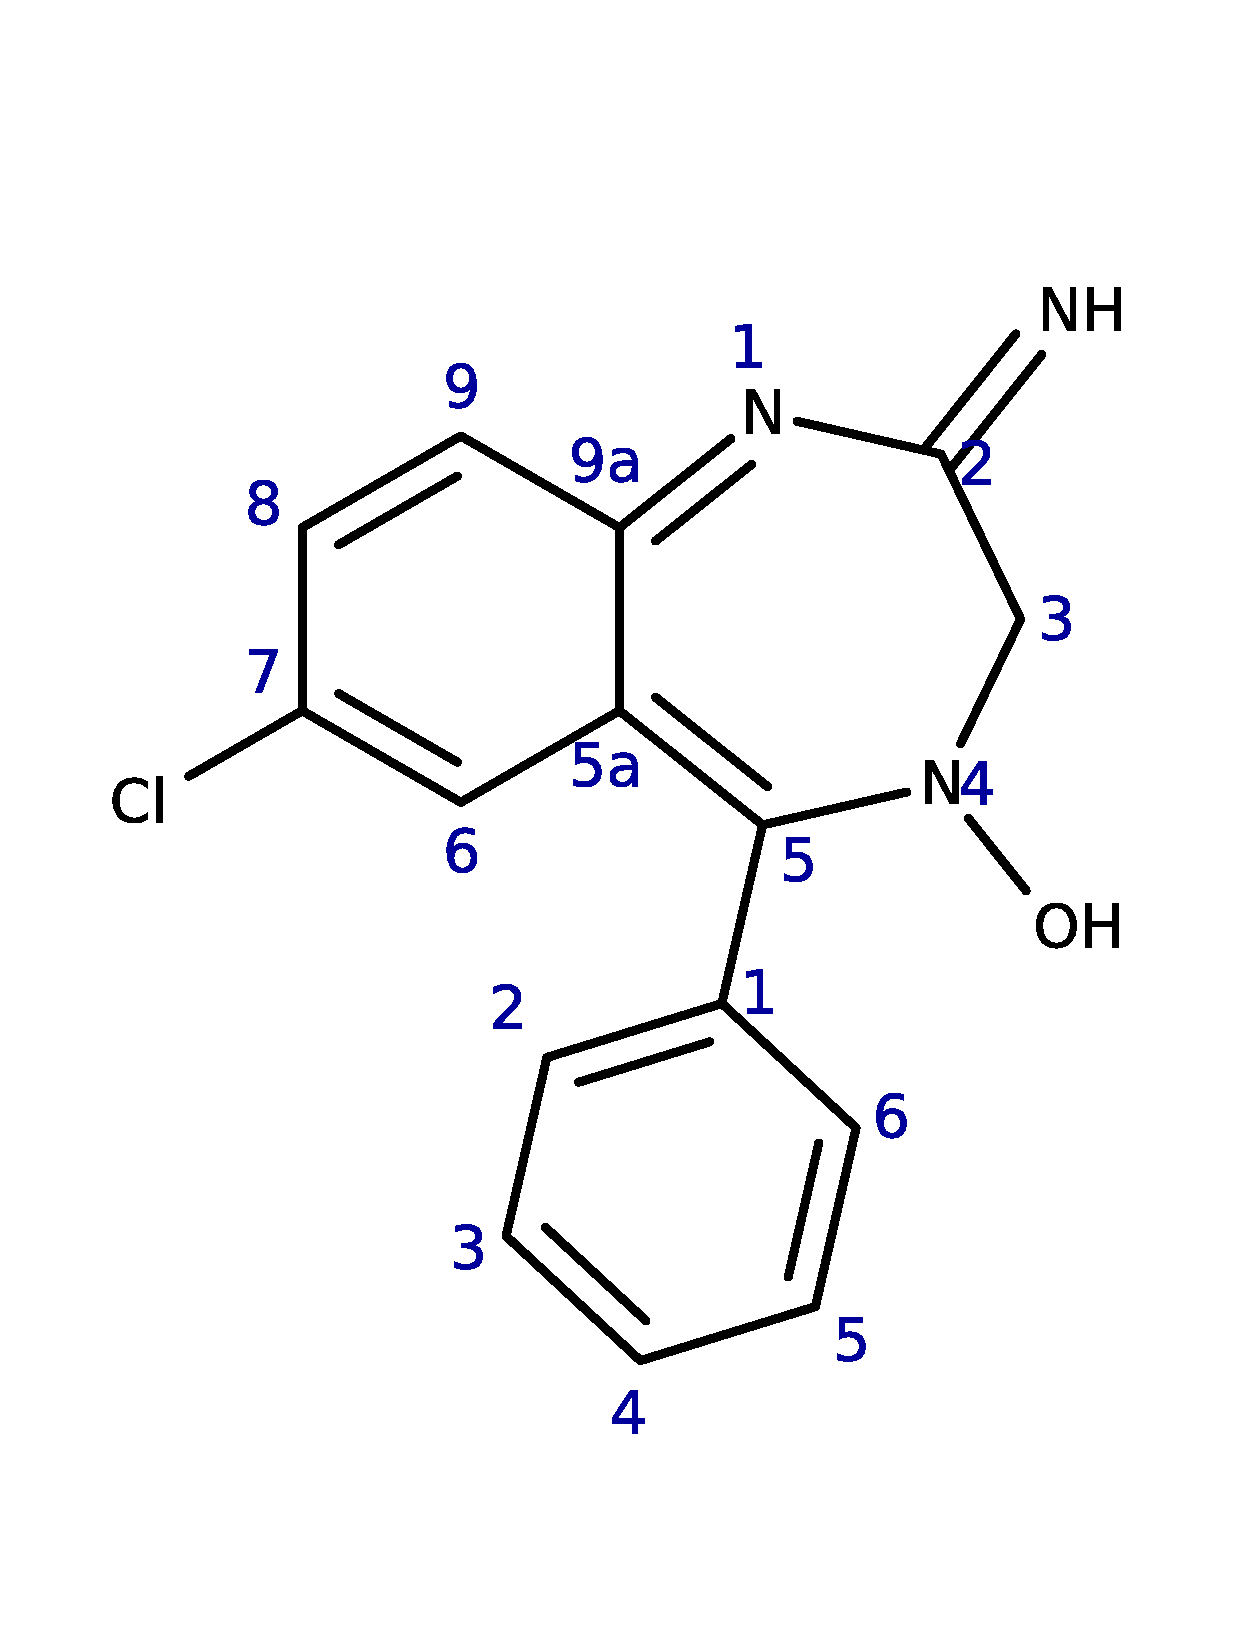
\includegraphics[width=\linewidth]{DesmethylChlordiazepoxide.pdf}
		\captionof{figure}{Desmethylchloridiazepoxide}
		\label{fig:desmeth}
	\end{minipage}%
	\begin{minipage}{0.5\textwidth}
		\centering
		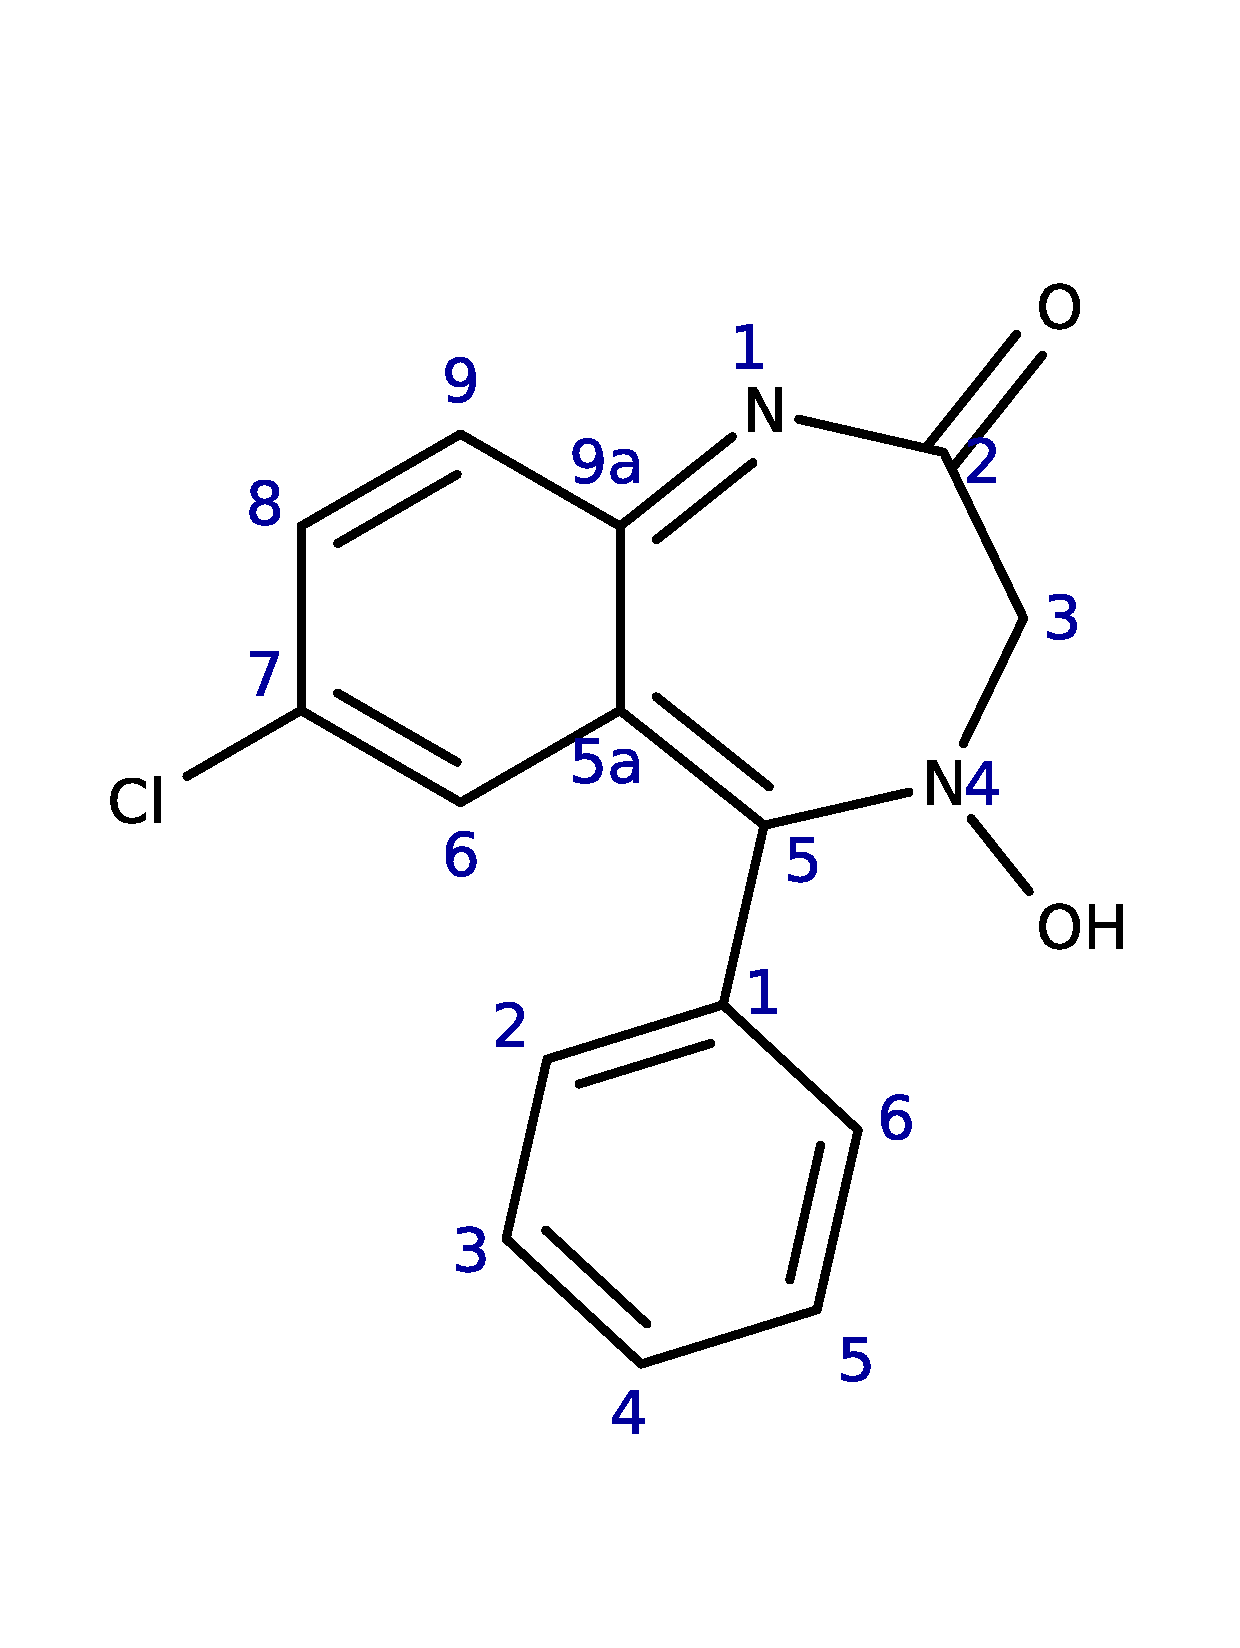
\includegraphics[width=\linewidth]{Demoxepam.pdf}
		\captionof{figure}{Demoxepam}
		\label{fig:demoxepam}
	\end{minipage}
\end{figure}

\begin{figure}[h]
	\centering
	\begin{minipage}{0.5\linewidth}
		\centering
		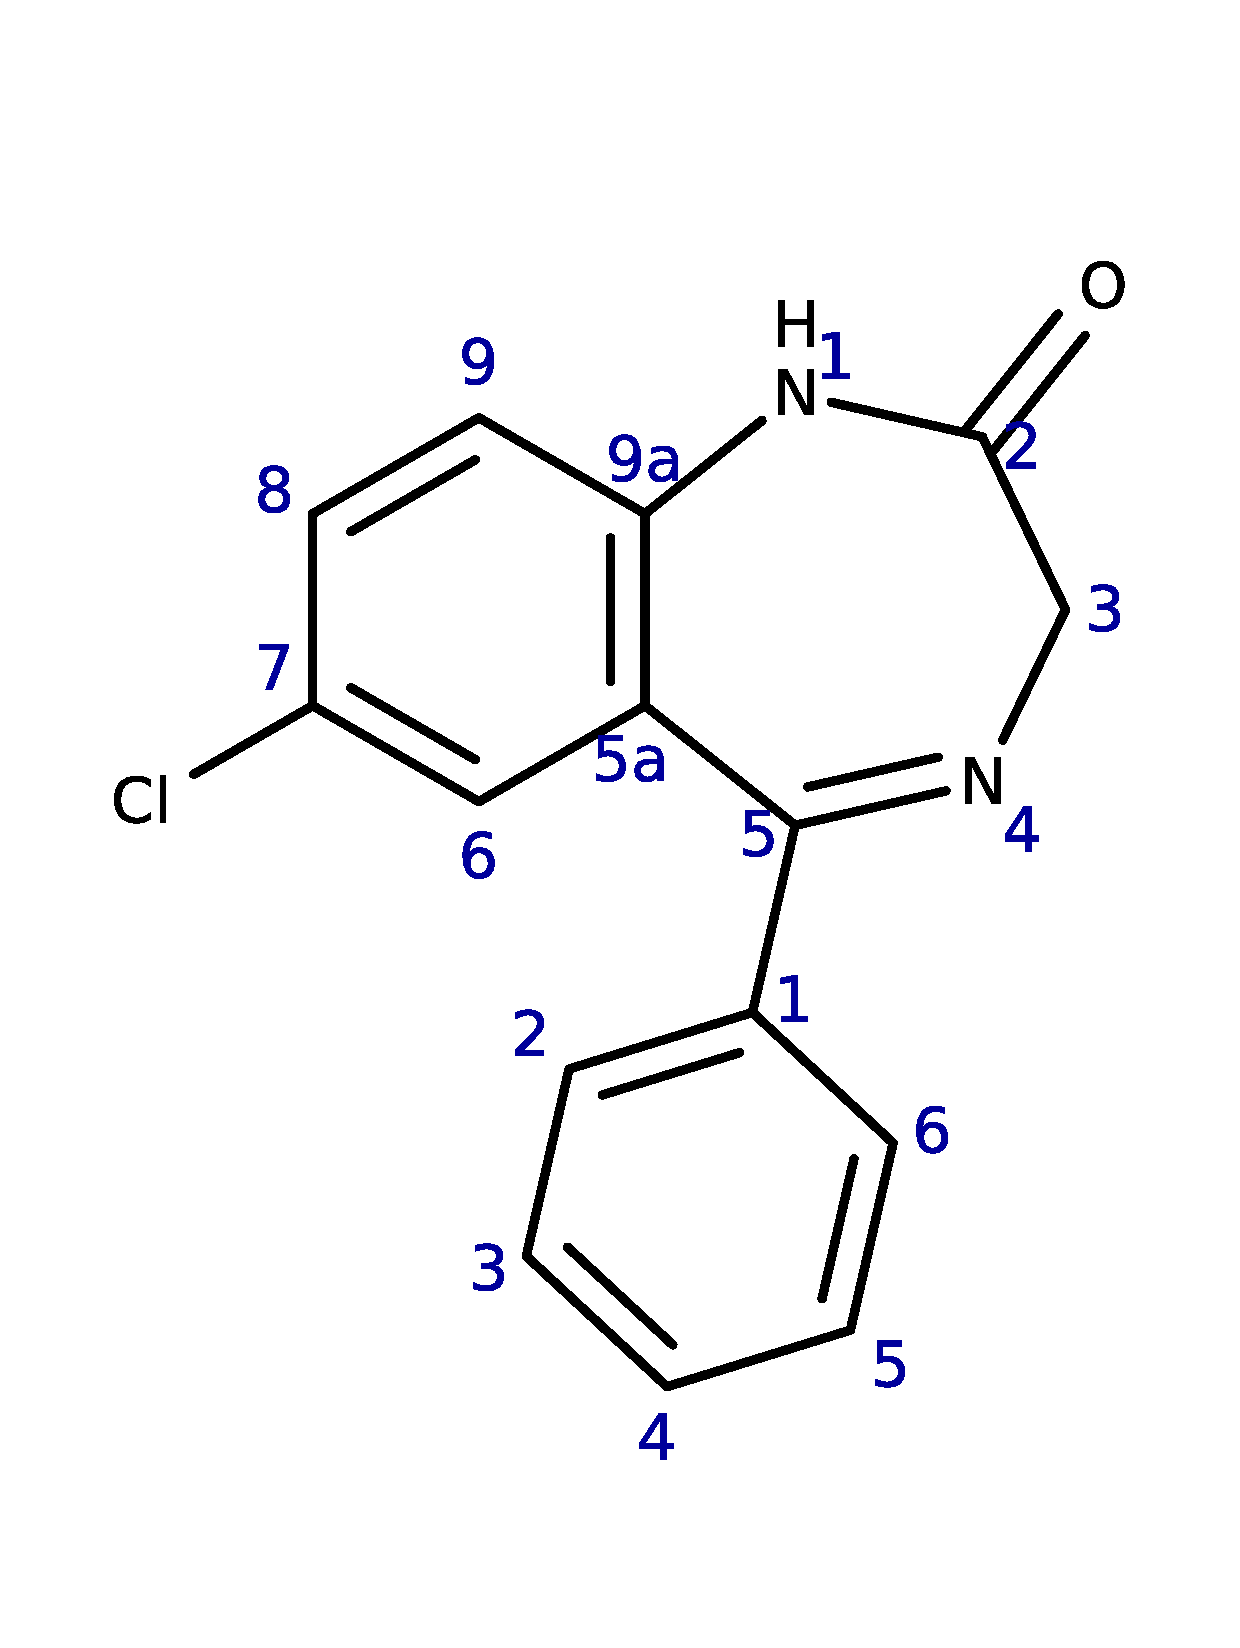
\includegraphics[width=\linewidth]{desmethyldiazepam.pdf}
		\captionof{figure}{Desmethyldeiazepam}
		\label{fig:desmethyldiazepam}
	\end{minipage}%
	\begin{minipage}{0.5\textwidth}
		\centering
		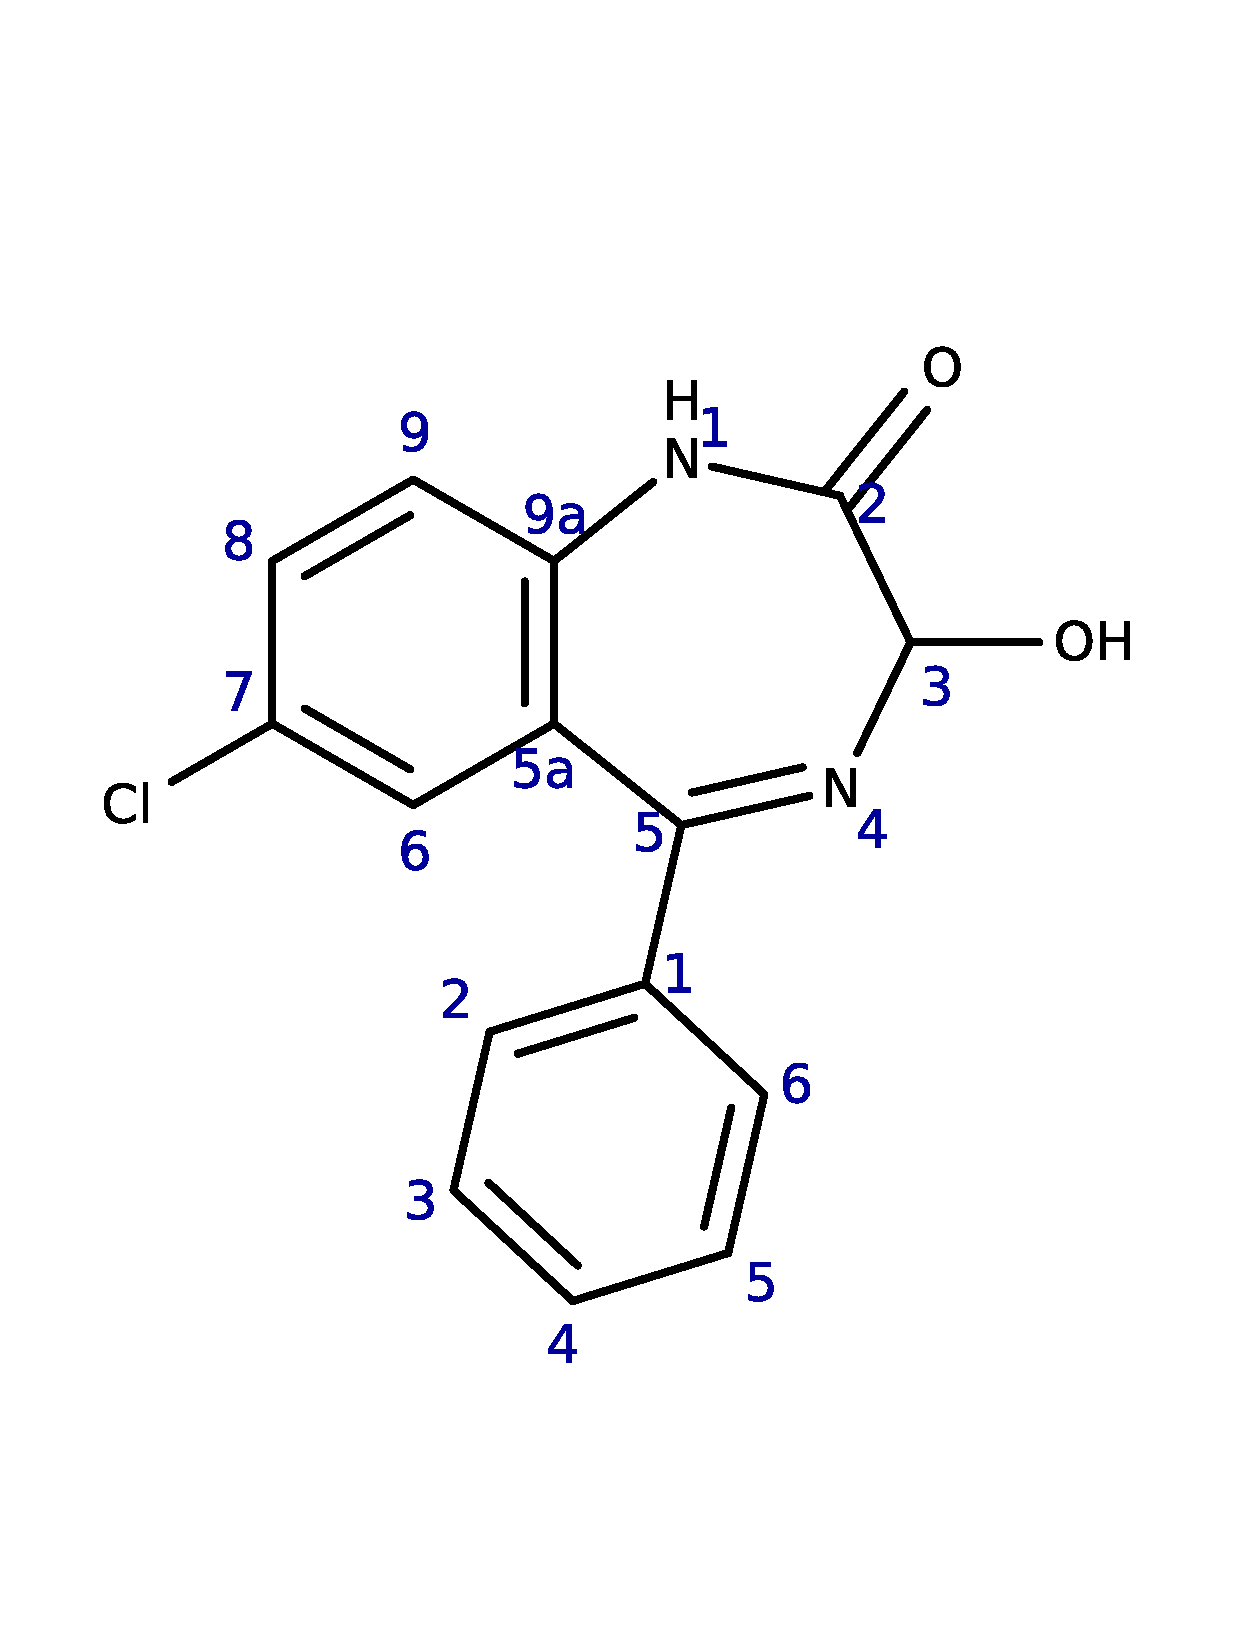
\includegraphics[width=\linewidth]{oxazepam.pdf}
		\captionof{figure}{Oxazepam}
		\label{fig:oxazepam}
	\end{minipage}
\end{figure}


\section{Diazepam}
 	The main active metabolite is desmethyldiazepam \emph{Fig} \ref{fig:desmethyldiazepam}, Along with inactive metabolites like temazepam \emph{Fig} \ref{fig:temazepam}, oxazepam \emph{Fig} \ref{fig:oxazepam}, and Nordiazepam O-glucuronide \emph{Fig} \ref{fig:norgluc}.\cite{RCM:RCM3613}

\begin{figure}[h]
	\centering
	\begin{minipage}{0.5\linewidth}
		\centering
		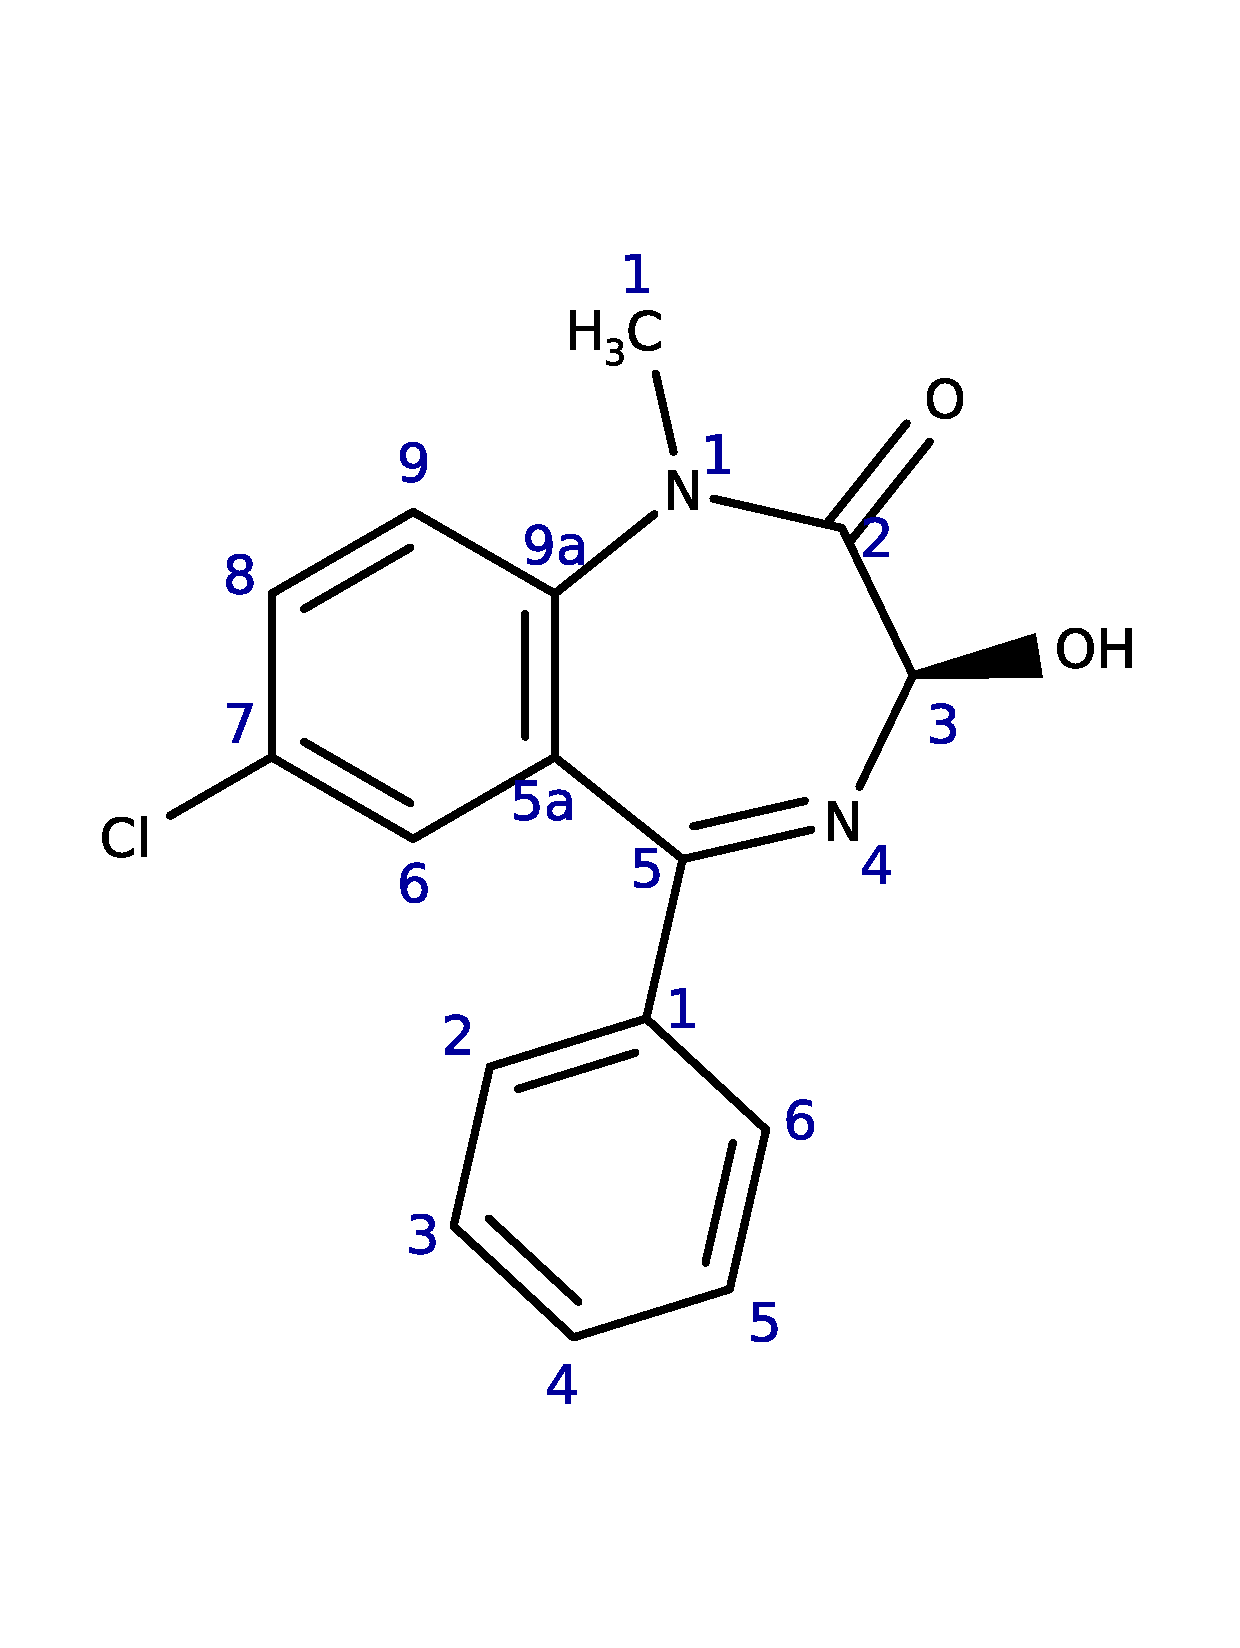
\includegraphics[width=\linewidth]{Temazepam.pdf}
		\captionof{figure}{Temazepam}
		\label{fig:temazepam}
	\end{minipage}%
	\begin{minipage}{0.5\textwidth}
		\centering
		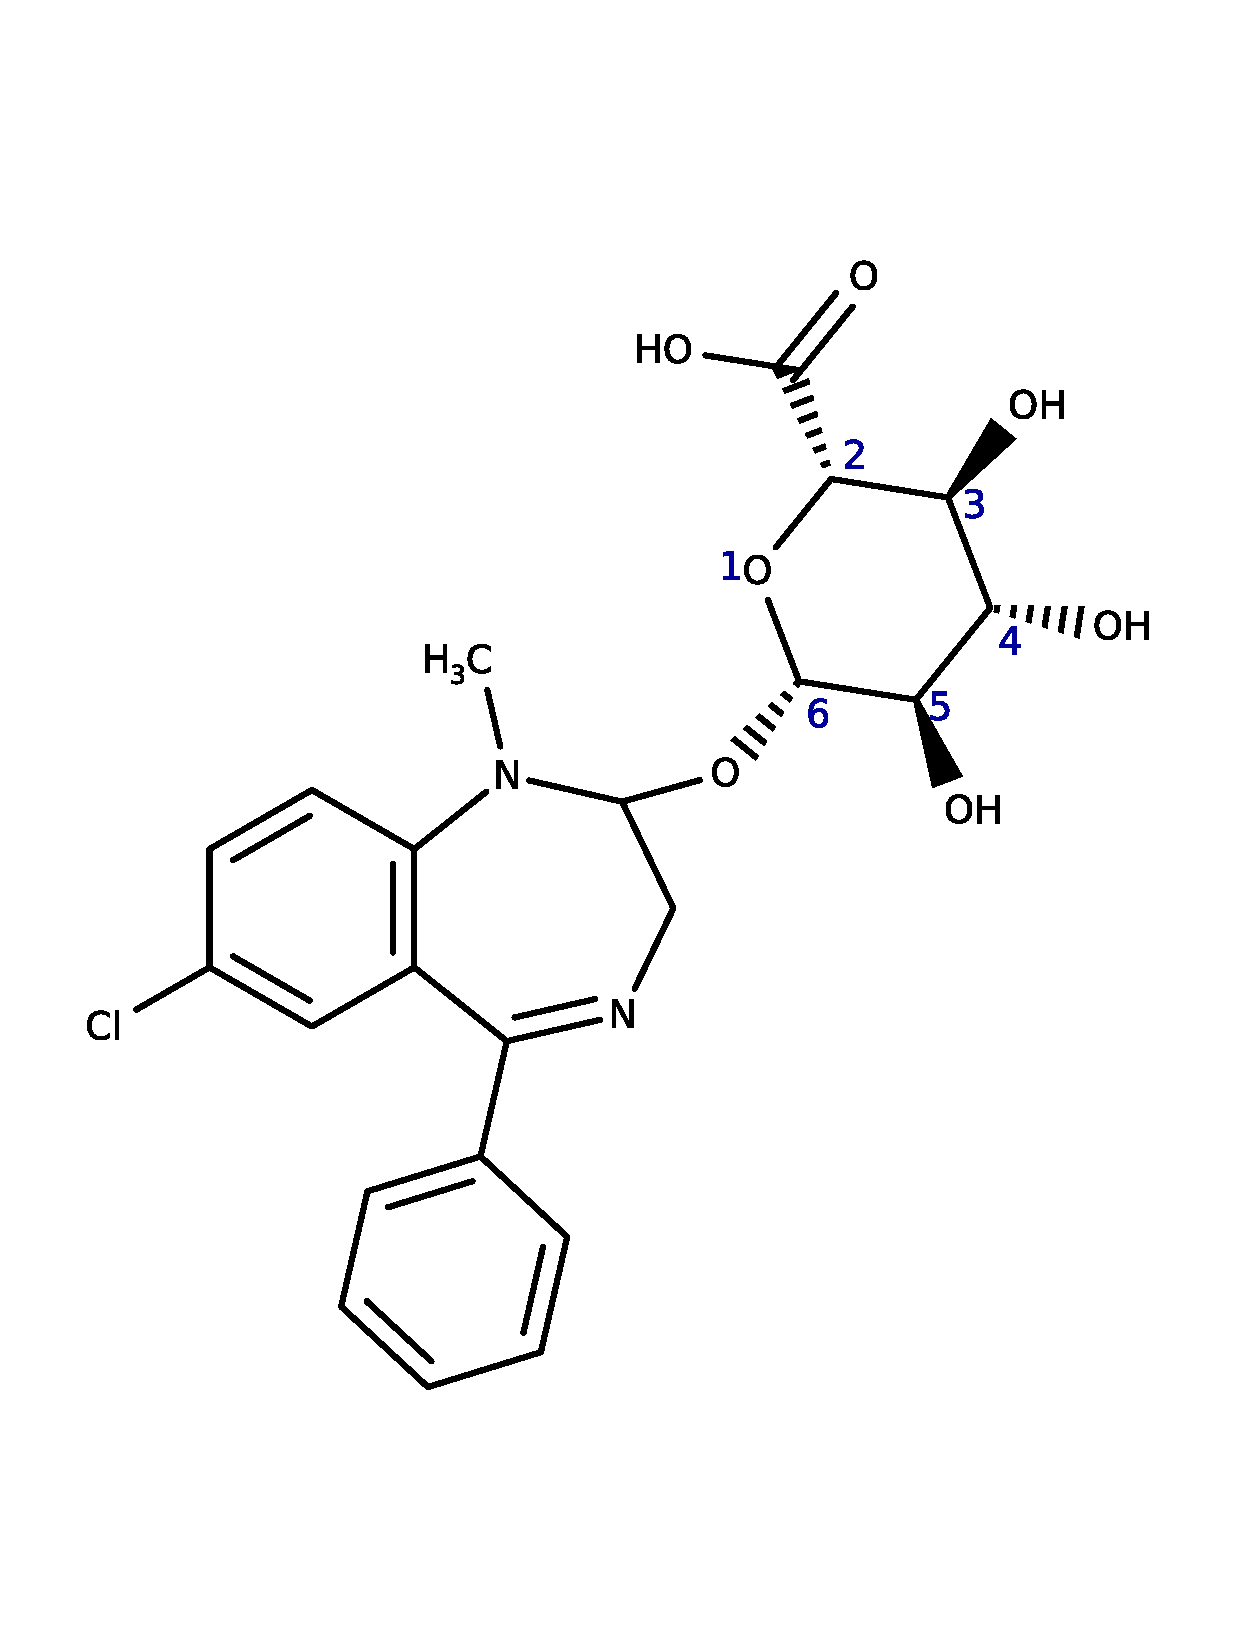
\includegraphics[width=\linewidth]{glucu.pdf}
		\captionof{figure}{Nordiazepam O-glucuronide}
		\label{fig:norgluc}
	\end{minipage}
\end{figure}





\section{Lorazepam} 
%The structure of the 3-0-phenolic glucuronie
Lorazepam is hepatically metabolized by conjugation to the 3-0-phenolic glucuronide which gives Lorazepam glucuronide \emph{Fig} \ref{fig:lorgluc}.\cite{elliott1976metabolism}

\begin{figure}[h]
	\centering
	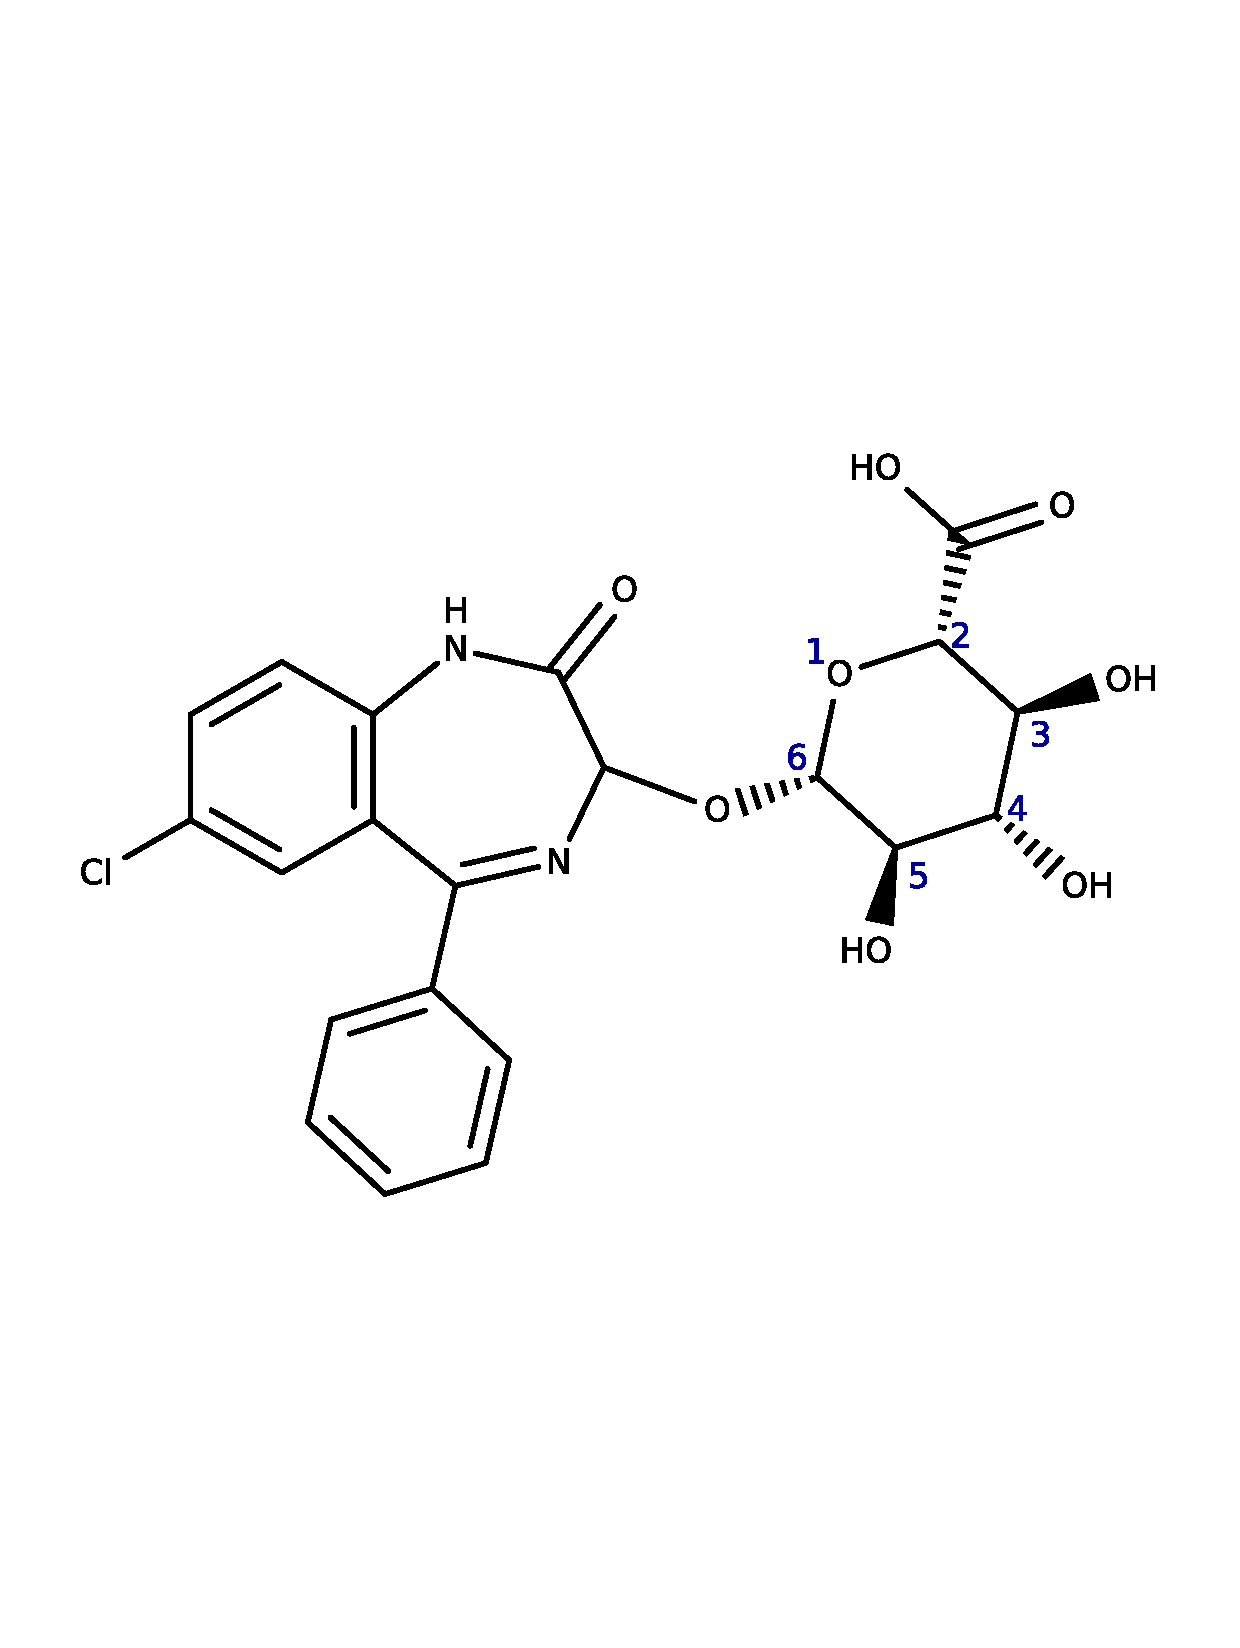
\includegraphics[width=\textwidth]{lorazapamglucu.pdf}
	\captionof{figure}{Nordiazepam O-glucuronide}
	\label{fig:lorgluc}
\end{figure}
